\documentclass[ASNA,twocolumn]{USG}

% ── Packages ─────────────────────────────────────────────────────
\usepackage{amsmath,amssymb}
\usepackage{booktabs}
\usepackage{graphicx}
\usepackage{xcolor}
\usepackage{hyperref}

\graphicspath{{./images/}{../../data/}{./figures/}}

% ── Metadata ──────────────────────────────────────────────────────
\articletype{RESEARCH ARTICLE}

\received{29 June 2026}
\revised{---}
\accepted{---}
\journal{Advanced Quantum Technologies}
\volume{0}
\copyyear{2026}
\startpage{1}

\begin{document}

\title{CrossEcho: Predictive Modelling of Crosstalk Side-Channel Leakage on Multi-Tenant Superconducting QPUs}

\author[1]{Justice Owusu Agyemang}
\author[1]{Jerry John Kponyo}
\author[1]{Elliot Amponsah}
\author[1]{Godfred Manu Addo Boakye}
\author[1]{Kwame Agyeman-Prempeh Agyekum}
\author[2]{Michael Agyare}

\authormark{Agyemang \textsc{et al.}}
\titlemark{CrossEcho: Predictive Modelling of Crosstalk Side-Channel Leakage}

\address[1]{\orgdiv{Quantum and Assistive Technologies Lab}, \orgname{Kwame Nkrumah University of Science and Technology}, %
\orgaddress{\city{Kumasi}, \country{Ghana}}}

\address[2]{\orgdiv{Ghana Communication Technology University}, %
\orgaddress{\city{Accra}, \country{Ghana}}}

\corres{Justice Owusu Agyemang (\email{justice.agyemang@knust.edu.gh})}

\fundingInfo{Institutional support from the Quantum and Assistive Technologies Lab, Kwame Nkrumah University of Science and Technology.}

\abstract[ABSTRACT]{%
Multi-tenant scheduling on cloud-based quantum processors introduces crosstalk---unwanted inter-qubit interactions that can be exploited as physical side-channels. While prior work has demonstrated that crosstalk leaks victim circuit information with high classification accuracy, all existing characterisations are post-hoc: they observe, fingerprint, or reconstruct the induced error after the attack executes. We present CrossEcho---named for the ``echo'' of a victim's gate operations imprinted on an attacker's qubits through the coupling fabric---a forward predictive model that forecasts crosstalk leakage magnitude from device calibration data, qubit placement, and circuit properties before measurement. The model derives effective ZZ coupling strengths from transmon perturbation theory, propagates calibration uncertainty via Monte Carlo sampling ($n=1000$), and is evaluated using a dual hold-out protocol ($33\%$ of qubit placements held out) on $46$ cells across two IBM Quantum Heron~r2 processors. A dedicated readout-only control experiment---the victim circuit has zero gates---isolates measurement-induced crosstalk from gate-induced ZZ coupling via their qualitatively different distance-decay signatures. The gate-crosstalk excess over the readout baseline is small but statistically significant ($p = 0.03$, Cohen's $d = 0.78$), requiring aggregate analysis for reliable detection. Cross-architecture validation on the Origin Quantum Cloud WK\_C180\_2 processor reveals an order-of-magnitude increase in crosstalk magnitude relative to IBM, directly confirming the architecture-dependence that the model identifies as its dominant uncertainty source. We establish the readout-only control as essential methodology for multi-tenant crosstalk studies, quantify the shot-count and circuit-depth thresholds needed to isolate the ZZ signal, and propose coarse frequency binning by cloud providers as a practical path to deployable forward crosstalk risk assessment.}

\keywords{crosstalk side-channel | multi-tenant QPU security | superconducting transmon | ZZ coupling | perturbation theory | readout crosstalk | predictive modelling | IBM Quantum | Origin Quantum Cloud}

\abbr{NISQ, Noisy Intermediate-Scale Quantum; QPU, Quantum Processing Unit; TVD, Total Variation Distance; ZZ, $|11\rangle \leftrightarrow |00\rangle$ diagonal coupling; QPT, Quantum Process Tomography; SWAP, exchange interaction path; RMSE, Root-Mean-Square Error; ECR, Echoed Cross-Resonance.}

\maketitle

% ===========================================================================
\section{Introduction}
\label{sec:introduction}

Cloud-based access to superconducting quantum processing units (QPUs) has become the dominant model for near-term quantum computing, following Preskill's NISQ paradigm~\cite{preskill2018nisq}. IBM Quantum, Amazon Braket, and Origin Quantum Cloud offer shared, queue-based access to processors with $100$--$1000+$ qubits~\cite{arute2019supremacy,ibmq2026,originqc2026}. To maximise hardware utilisation, these platforms increasingly adopt multi-tenant scheduling where circuits from independent users execute concurrently on different regions of the same physical chip~\cite{tannu2019qubits,murali2019fullstack}.

This architectural choice introduces a security vulnerability rooted in the physics of superconducting qubits. Transmons are coupled through shared bus resonators and parasitic capacitances~\cite{koch2007transmon,krantz2019guide}, producing a static ZZ interaction---a diagonal coupling between computational states arising from weak anharmonicity~\cite{ding2020crosstalk,sarovar2020detecting}. When an attacker's and victim's circuits execute on adjacent qubits, each two-qubit gate in the victim's circuit accumulates a ZZ phase on the attacker's qubits. This phase---an ``echo'' of the victim's operations propagating through the coupling fabric---can be detected in the attacker's measurement statistics, constituting a physical side-channel. The project name CrossEcho reflects this mechanism: crosstalk across the coupling topology creates an echo of one user's computation in another user's measurement outcomes.

The security community has demonstrated that this mechanism is practically exploitable. Hu~\emph{et al.}~\cite{hu2025swap} showed that a single CNOT gate from an attacker can reduce a victim Grover algorithm's accuracy by $81.62\%$; a passive probe occupying $6.25\%$ of the victim's qubits predicted circuit size with $100\%$ accuracy. Choudhury~\emph{et al.}~\cite{choudhury2024crosstalk} applied graph-based learning to crosstalk-inferred CNOT signatures, achieving $85.7\%$ algorithm classification across $336$ benchmark circuits. Shubha and Farheen~\cite{shubha2025pulse} built an end-to-end pulse-to-circuit characterisation framework using quantum process tomography (QPT) and isometry-based circuit extraction, reconstructing the logical error channel post-hoc. Harper~\emph{et al.}~\cite{harper2025crosstalk}---published in this journal---characterised crosstalk via tomography and evaluated three mitigation strategies. Coupel and Farheen~\cite{coupel2025survey} catalogued the quantum cloud vulnerability landscape, and Das and Ghosh~\cite{das2025calibration} demonstrated adversarial calibration misreporting on IBM hardware.

\textbf{The gap across all prior work is methodological.} Every existing study characterises or exploits crosstalk \emph{empirically}: execute the attack, observe the outcome, classify or reconstruct it. None provide a forward predictive model---one that takes device calibration data, qubit placement, and circuit properties as input and outputs a \emph{forecasted} leakage magnitude with calibrated uncertainty, evaluated on genuinely unseen configurations. This distinction---post-hoc characterisation versus forward prediction---mirrors the historical development of classical cloud security, where the progression from empirical co-residency detection~\cite{ristenpart2009hey} to analytical information-leakage models was essential for enabling pre-deployment risk assessment. The quantum multi-tenant community needs the same progression, and CrossEcho is a step in that direction.

This paper makes four contributions:

\begin{enumerate}
    \item \textbf{A forward model of crosstalk leakage} derived from first-principles transmon perturbation theory (Section~\ref{sec:model}). Given calibration data accessible through standard cloud APIs (T1, T2, coupling map, gate errors), attacker--victim placement, and victim two-qubit gate density, the model computes effective ZZ coupling along the shortest SWAP path, predicts total variation distance via phase accumulation, and provides confidence intervals through Monte Carlo uncertainty propagation ($n=1000$). The model is validated against published direct measurements of ZZ coupling in fixed-frequency transmon lattices. The full pipeline from calibration to evaluation is illustrated in Figure~\ref{fig:flowchart}.

    \item \textbf{A readout-only control experiment}---to our knowledge the first dedicated control for isolating measurement crosstalk in a multi-tenant side-channel context (Section~\ref{sec:methods}). The victim circuit has zero gates; any measured leakage is purely readout crosstalk. This control disambiguates the two crosstalk mechanisms, which produce qualitatively different distance-decay signatures: gate-induced ZZ coupling decays exponentially with SWAP-path distance ($d_0 \approx 1$--$2$ hops), while readout crosstalk, mediated by the shared measurement infrastructure, is approximately distance-independent.

    \item \textbf{Dual hold-out evaluation on real quantum hardware} across two superconducting architectures and three processors (Section~\ref{sec:results}). On IBM Quantum ($46$ cells, $2000$ shots/cell), we forecast on $33\%$ held-out placement configurations. Cross-architecture validation on Origin WK\_C180\_2 reveals an order-of-magnitude increase in crosstalk, directly confirming architecture dependence. We report proper statistical characterisation ($t$-test, Cohen's $d$, confidence intervals) throughout.

    \item \textbf{A systematic error budget and deployment roadmap} (Section~\ref{sec:discussion}) that identifies the dominant uncertainty source---frequency opaqueness in the cloud API---and proposes coarse frequency binning as a practical, IP-preserving mitigation that would reduce model error by $\sim 90\%$ and enable deployable pre-submission crosstalk risk assessment.
\end{enumerate}

% ===========================================================================
\section{Background and Related Work}
\label{sec:related}

\subsection{Transmon Physics and ZZ Crosstalk}

The transmon qubit, introduced by Koch~\emph{et al.}~\cite{koch2007transmon} and comprehensively reviewed by Krantz~\emph{et al.}~\cite{krantz2019guide}, is the dominant superconducting qubit architecture because its weak anharmonicity $\alpha = -E_C \approx -200$ to $-350$~MHz suppresses charge noise while providing the non-linearity needed for a computational two-level system. The trade-off is that the higher transmon levels ($|2\rangle, |3\rangle, \ldots$) introduce static ZZ coupling between capacitively coupled qubit pairs---an always-on diagonal interaction that shifts the $|11\rangle$ state energy relative to the bare sum of individual qubit frequencies. This shift is not an engineering defect; it is a direct consequence of the Duffing-oscillator nonlinearity that makes the transmon a qubit.

The physics community has studied ZZ coupling extensively as a noise source. Ding~\emph{et al.}~\cite{ding2020crosstalk} systematically demonstrated that deliberate qubit frequency assignments---frequency-aware compilation---can suppress ZZ coupling by orders of magnitude, by ensuring that no pair of coupled qubits has a detuning $\Delta$ close to the anharmonicity $\alpha$ where ZZ coupling diverges (Eq.~\ref{eq:zz_simplified}). Sarovar~\emph{et al.}~\cite{sarovar2020detecting} developed randomised-benchmarking protocols for detecting crosstalk errors in multi-qubit processors. Wei~\emph{et al.}~\cite{wei2022characterizing} provided the first comprehensive experimental characterisation of crosstalk magnitudes in transmon processors. Osman~\emph{et al.}~\cite{osman2023mitigation} demonstrated a fabrication-level approach: larger Josephson junctions with $2\%$ resistance standard deviation achieve $40$~MHz frequency spread across $32$ identical transmons with quality factors exceeding $2\times10^6$, reducing frequency collisions at the hardware level. Alghadeer~\emph{et al.}~\cite{alghadeer2025low,alghadeer2025crosstalk} characterised crosstalk dispersion and spatial scaling in fixed-frequency transmon lattices, demonstrating a $16$-qubit tileable architecture with suppressed parasitic coupling, and developed a capacitance-matrix localisation framework with evanescent field decay models that quantitatively predicted nearest-neighbour couplings. Their directly measured ZZ values ($8$--$35$~kHz) provide the experimental validation benchmark we use for our perturbation-theory model (Section~\ref{sec:model}).

Crucially, none of these physics and engineering studies frame crosstalk as a security problem. They treat it as a noise source to be characterised and mitigated---an entirely appropriate framing for single-user quantum computation. Our contribution is to re-frame the same perturbation-theory physics as an \emph{information channel} between adversarial users sharing a QPU. The model is the same; the question it answers is different: not ``how much error does crosstalk add?'', but ``how much information about the victim does crosstalk leak?''

\subsection{Multi-Tenant Quantum Security}

The multi-tenant quantum security threat was first systematically articulated by Tannu and Qureshi~\cite{tannu2019qubits}, who demonstrated that qubit-to-qubit variability in coherence times and gate fidelities creates security-relevant allocation policies: placing a victim on ``good'' qubits and an attacker on ``bad'' qubits is not a defence if the attacker can choose which qubits to request. Murali~\emph{et al.}~\cite{murali2019fullstack} provided the first full-stack study of architectural implications of multi-tenancy on real quantum systems, including scheduling, qubit allocation, and noise-aware compilation.

Four recent works directly demonstrate crosstalk-based side-channel attacks, forming the immediate context for CrossEcho:

\textit{Attack demonstration.} Hu~\emph{et al.}~\cite{hu2025swap} identified the SWAP path between qubits as the root cause of crosstalk leakage and demonstrated active attacks (Grover accuracy reduced by $81.62\%$ from a single strategically placed CNOT) and passive attacks ($100\%$ circuit-size prediction accuracy from a probe occupying only $6.25\%$ of the victim's qubit count) on IBM hardware. This work established that the threat is real and exploitable at NISQ scales.

\textit{Machine-learning fingerprinting.} Choudhury~\emph{et al.}~\cite{choudhury2024crosstalk} treated crosstalk-inferred CNOT gate signatures as features for a graph-learning classifier, achieving $85.7\%$ algorithm identification accuracy across $336$ benchmark circuits. This demonstrated that machine learning can amplify small crosstalk signatures into high-accuracy classification, even when individual measurements are noisy.

\textit{Post-hoc channel reconstruction.} Shubha and Farheen~\cite{shubha2025pulse}---the closest prior work---built a pulse-to-circuit pipeline: density-matrix simulation of the physical attack, followed by full quantum process tomography (QPT) and novel isometry-based circuit extraction to reconstruct the induced logical error channel from the physical pulse sequence. Their framework is the most complete crosstalk characterisation to date and identifies an asymmetric two-qubit adversarial mechanism (driver $+$ catalyst). However, it is fundamentally post-hoc: it reconstructs what \emph{did} happen after executing the attack. It requires running the attack and performing full QPT---an exponential-cost procedure---for each placement configuration of interest.

\textit{Defence evaluation.} Harper~\emph{et al.}~\cite{harper2025crosstalk}, published in this journal, provided the first thorough experimental characterisation of crosstalk as an attack vector and evaluated three mitigation strategies (circuit separation, RL-based qubit allocation, and spectator qubits), finding all three overcome crosstalk attacks with varying degrees of success.

\textbf{The key differentiator.} Hu, Choudhury, and Harper observe and empirically fingerprint leakage. Shubha and Farheen reconstruct the error channel post-hoc via QPT. None provide a forward model. CrossEcho predicts leakage from calibration data \emph{before} measurement, enabling pre-submission risk quantification---the quantum analogue of static analysis in classical software security~\cite{ristenpart2009hey}---rather than post-hoc forensic analysis. This is not an incremental improvement; it is a different class of tool.

\subsection{Readout Crosstalk and Measurement Physics}

The distinction between gate-induced ZZ crosstalk and measurement-induced readout crosstalk is fundamental to our experimental design and, we argue, to the interpretation of all published multi-tenant crosstalk results.

Dispersive readout~\cite{sank2016measurement,heimsoo2018rapid} couples each transmon qubit to a dedicated readout resonator whose frequency shifts by the qubit-state-dependent cavity pull $\chi$. During measurement, the resonator is interrogated via a common feedline shared by multiple qubits. Three mechanisms contribute to readout crosstalk: (i) parasitic microwave coupling between adjacent readout resonators on the same feedline~\cite{mitigating2025measurement}; (ii) classical crosstalk in the Josephson parametric amplifier (JPA) chain that amplifies the readout signal before room-temperature digitisation; and (iii) residual coupling in the IQ mixer and analogue-to-digital converter (ADC) paths.

Unlike ZZ coupling, which is a qubit-qubit interaction propagating along the coupling graph and decaying exponentially with distance ($d_0 \approx 1$--$2$ hops via Eq.~\ref{eq:swap_path}), readout crosstalk is mediated by the frequency-multiplexed classical measurement infrastructure and is approximately independent of the coupling-graph distance between qubits. This qualitative difference in distance-decay signatures is the basis for our control experiment: flat distance decay implicates readout crosstalk; exponential decay with $d_0 \approx 1$--$2$ hops implicates gate-induced ZZ coupling.

Kumar~\emph{et al.}~\cite{timeadaptive2025crosstalk} recently proposed a time-adaptive single-shot crosstalk detector using spectator qubits and multiple quantum coherence, achieving $85$--$93\%$ detection probability for random crosstalk events. Their detector-based approach complements our predictive approach: detection identifies crosstalk after it occurs, while prediction estimates risk before circuits are submitted.

% ===========================================================================
\section{Threat Model}
\label{sec:threat}

We formalise the multi-tenant crosstalk threat as a distinguishing game between two hypotheses about the environment in which the attacker's circuit executes.

\subsection{System Model}

A cloud-based superconducting QPU with $N_q$ qubits is shared by two users: a victim (Alice) and an attacker (Eve). The provider's scheduler allocates disjoint qubit subsets $\mathcal{V} \subset \{0,\ldots,N_q-1\}$ and $\mathcal{A} \subset \{0,\ldots,N_q-1\}$ to Alice and Eve, respectively, with $\mathcal{V} \cap \mathcal{A} = \emptyset$. The coupling graph $G = (Figure~\ref{fig:threat_model}) (\{0,\ldots,N_q-1\}, E)$---published by the provider---specifies which qubit pairs are capacitively coupled. The distance $d(\mathcal{A}, \mathcal{V})$ is the minimum number of coupling-graph hops between any qubit in $\mathcal{A}$ and any qubit in $\mathcal{V}$.

Alice submits a quantum circuit $C_V$ on qubits $\mathcal{V}$ with two-qubit gate density $\rho_{\mathrm{2Q}}$ and depth $D$. Eve submits a quantum circuit $C_A$ on qubits $\mathcal{A}$ with sensitivity factor $s$ ($s=1$ for idle probes, $s=2$ for CNOT probes). Both circuits execute within the same scheduling window. After execution, Eve receives $N$ measurement outcomes $\{x_i\}_{i=1}^N$ from her qubits, drawn i.i.d.\ from the distribution $P_{\mathcal{A}} = \mathrm{diag}_{\mathcal{A}}(\mathrm{Tr}_{\overline{\mathcal{A}}}[\rho_{\mathrm{out}}])$ where $\rho_{\mathrm{out}}$ is the output state of the combined $C_V \otimes C_A$ evolution followed by computational-basis measurement on $\mathcal{A}$.

\subsection{Attacker Capabilities and Distinguishing Game}

Eve controls $C_A$ (qubit indices within $\mathcal{A}$, gate sequence, shot count $N$) exclusively through the standard cloud SDK. She has no elevated privileges: no pulse-level access, no calibration data beyond what the SDK exposes (T1, T2, gate errors, readout errors, and the coupling map), and no ability to interfere with Alice's job submission, execution, or result retrieval. She observes $\{x_i\}_{i=1}^N$ and nothing else.

Eve plays a distinguishing game with two hypotheses:
\begin{align}
    \mathcal{H}_0 &: \text{Alice is running circuit } C_V \text{ (victim present)}, \\
    \mathcal{H}_1 &: \text{Alice is idle (victim absent)}.
\end{align}
From her $N$ samples, Eve constructs an empirical distribution $\hat{P}_{\mathcal{A}} = \frac{1}{N}\sum_{i=1}^N \delta_{x_i}$ and computes a test statistic. The optimal distinguishability between the two hypotheses from a single measurement is bounded by the total variation distance between the underlying distributions~\cite{preskill2018nisq}:
\begin{equation}
    \mathrm{TVD}(P_{\mathcal{A}}^{\mathcal{H}_0}, P_{\mathcal{A}}^{\mathcal{H}_1}) \leq \sup_{\text{test}} |\Pr[\text{accept } \mathcal{H}_0|\mathcal{H}_0] - \Pr[\text{accept } \mathcal{H}_0|\mathcal{H}_1]|.
\end{equation}
TVD therefore quantifies the maximum single-shot information leakage from Alice's circuit to Eve's measurement statistics. With $N$ independent measurements, the distinguishing advantage scales as $\sim \sqrt{N} \cdot \mathrm{TVD}$ (by Neyman--Pearson). Eve's goal is to infer properties of $C_V$ (two-qubit gate presence, circuit depth, algorithm class) from these statistics, as established in prior work~\cite{hu2025swap,choudhury2024crosstalk}.

\subsection{Defender Model and Attack Assumptions}

The cloud provider applies standard qubit allocation and may employ frequency engineering~\cite{ding2020crosstalk,osman2023mitigation} to suppress ZZ coupling, but does not actively monitor for crosstalk attacks or apply runtime countermeasures. We assume collective attacks: Eve's interaction with each round of the combined $C_V \otimes C_A$ evolution is independent and identically distributed, justified by the absence of quantum memory in current superconducting processors.

Our contribution is not a new attack. It is a predictive framework that, given a calibration snapshot and a proposed $(\mathcal{V}, \mathcal{A}, C_V)$ configuration, outputs a forecasted TVD value with uncertainty $\sigma_L$---the quantity Eve needs to optimise her probe placement, and the quantity the provider needs to assess scheduling risk. The framework is symmetric: it serves both attacker and defender.

\begin{figure}[t]
\centering
\begin{tikzpicture}[
    box/.style={rounded corners=2pt, draw=#1!60, fill=#1!15, text width=2.2cm, align=center, font=\footnotesize, inner sep=4pt},
    qbox/.style={draw=#1!70, fill=white, minimum size=0.45cm, font=\tiny, rounded corners=1pt, line width=0.6pt},
    arrow/.style={->, >=stealth, semithick},
    annot/.style={font=\scriptsize\itshape},
]
% Chip background
\fill[gray!5, rounded corners=4pt] (-0.2,-0.45) rectangle (7.6,1.5);
\node[font=\scriptsize] at (3.7,1.75) {Multi-Tenant Superconducting QPU};

% ── SWAP path drawn FIRST so it sits behind qubit boxes ──
\draw[orange!70, line width=2.2pt, opacity=0.5, rounded corners=2pt]
    (1.85,0.6) -- (2.55,0.6) -- (3.25,0.6) -- (3.95,0.6) -- (4.65,0.6) -- (5.45,0.6);
\node[annot, orange!80] at (3.7,1.2) {SWAP path ($d=5$)};

% Qubit boxes (drawn AFTER SWAP path, on top)
% Victim
\node[qbox=blue] (v0) at (0.3,0.55) {$q_0$};
\node[qbox=blue] (v1) at (1.05,0.55) {$q_1$};
\node[qbox=blue] (v2) at (1.8,0.55) {$q_2$};
% Intermediate
\node[qbox=black!40] (m0) at (2.55,0.55) {$q_3$};
\node[qbox=black!40] (m1) at (3.3,0.55) {$q_4$};
\node[qbox=black!40] (m2) at (4.05,0.55) {$q_5$};
\node[qbox=black!40] (m3) at (4.8,0.55) {$q_6$};
% Attacker
\node[qbox=red] (a0) at (5.55,0.55) {$q_7$};
\node[qbox=red] (a1) at (6.3,0.55) {$q_8$};

% Region outlines (drawn before qubit nodes so they sit behind)
\draw[blue!50, thick, rounded corners] (-0.15,-0.25) rectangle (2.1,1.15);
\draw[red!50, thick, rounded corners] (5.3,-0.25) rectangle (6.55,1.15);
\node[font=\scriptsize, blue!70] at (0.95,1.4) {Alice (victim) $\mathcal{V}$};
\node[font=\scriptsize, red!70] at (5.9,1.4) {Eve $\mathcal{A}$};

% Coupling edges (drawn before qubit nodes)
\draw[gray!30, thin] (v0) -- (v1) -- (v2);
\draw[gray!30, thin] (v2) -- (m0) -- (m1) -- (m2) -- (m3);
\draw[gray!30, thin] (m3) -- (a0) -- (a1);

% ── Below chip: Eve's observation chain ──
% Both qubits converge to a junction, then a single arrow to measurement
\coordinate (junction) at (5.9,-0.15);
\draw[arrow, red!60] (a0.south) -- ++(0,-0.25) -| (junction);
\draw[arrow, red!60] (a1.south) -- ++(0,-0.25) -| (junction);

\node[box=red, text width=2.2cm] (meas) at (5.9,-1.2) {Eve's Measurement\\$\{x_i\}_{i=1}^N$};
\draw[arrow, red!60] (junction) -- (meas.north);

% Distinguishing game below measurement
\node[box=gray, text width=2.2cm] (game) at (5.9,-2.5) {Distinguishing Game\\$\mathcal{H}_0{:}C_V$ vs.\ $\mathcal{H}_1{:}$idle};
\draw[arrow, red!60] (meas.south) -- (game.north);

\end{tikzpicture}
\caption{Threat model. Alice occupies qubit region $\mathcal{V}$ (blue outline); Eve occupies $\mathcal{A}$ (red outline). Individual qubits are white with colored borders. The coupling fabric (grey-outlined qubits) connects the regions. The SWAP path (orange band, drawn behind qubits) mediates the effective ZZ interaction $\zeta_{\mathrm{eff}}$. Eve's measurement outcomes (aggregated from both attacker qubits) feed a distinguishing game.}
\label{fig:threat_model}
\end{figure}

% ===========================================================================
\section{Analytic Leakage Model}
\label{sec:model}

\subsection{Transmon Hamiltonian and ZZ Coupling}

Each transmon qubit is a weakly anharmonic Duffing oscillator~\cite{koch2007transmon,krantz2019guide}:
\begin{equation}
    H_i = \omega_i a_i^\dagger a_i + \frac{\alpha_i}{2} a_i^\dagger a_i^\dagger a_i a_i,
\label{eq:transmon}
\end{equation}
with $\omega_i \approx 4.8$--$5.3$~GHz and $\alpha_i = -E_C \approx -200$ to $-350$~MHz. Capacitive coupling between adjacent qubits is $H_{ij} = g_{ij}(a_i^\dagger a_j + a_i a_j^\dagger)$ with $g_{ij} \approx 10$--$20$~MHz determined by the mutual capacitance $C_m$ and self-capacitances of the qubit islands.

Treating the coupling as a perturbation and computing dressed eigenstate energies to leading non-vanishing order yields the static ZZ coupling strength~\cite{ding2020crosstalk,sarovar2020detecting}:
\begin{equation}
    \zeta_{ij} = \frac{g^2}{\Delta_{ij} + \alpha_j} + \frac{g^2}{-\Delta_{ij} + \alpha_i},
\label{eq:zz_coupling}
\end{equation}
where $\Delta_{ij} = \omega_i - \omega_j$. For equal anharmonicities, this simplifies to:
\begin{equation}
    \zeta_{ij} = -\frac{2g^2\alpha}{\Delta_{ij}^2 - \alpha^2}.
\label{eq:zz_simplified}
\end{equation}

Equation~(\ref{eq:zz_simplified}) reveals the strong detuning dependence that underpins frequency-engineering-based crosstalk suppression. With conservative transmon parameters ($g = 20$~MHz, $\alpha = -300$~MHz): $|\zeta| \approx 4.8$~MHz at $\Delta = 200$~MHz versus $|\zeta| \approx 120$~kHz at $\Delta = 1$~GHz---a $40\times$ suppression. The denominator $\Delta^2 - \alpha^2$ vanishes when $|\Delta| = |\alpha| \approx 300$~MHz, producing a ZZ resonance that frequency engineering must avoid. IBM's Heron~r2 processors exploit this physics~\cite{ibmq2026}, maintaining $\Delta \gtrsim 500$~MHz across all coupled pairs to push $|\zeta|$ below $\sim 50$~kHz.

We validated the perturbation-theory formula against published direct measurements. Alghadeer~\emph{et al.}~\cite{alghadeer2025crosstalk} report measured nearest-neighbour ZZ coupling of $8$--$35$~kHz on a $4\times4$ fixed-frequency transmon lattice with $\Delta \approx 200$--$600$~MHz, after accounting for virtual coupling suppression via off-chip inductive shunting. Equation~(\ref{eq:zz_simplified}) with their reported parameters ($g \approx 5$--$12$~MHz, $\alpha \approx -250$~MHz, $\Delta \approx 200$--$600$~MHz) yields $|\zeta| \approx 3$--$45$~kHz, consistent within a factor of $\sim 2$. This agreement gives us confidence that perturbation theory captures the correct order of magnitude, with residual uncertainty dominated by the unobserved individual qubit frequencies and $g$ values.

\subsection{SWAP-Path Propagation}

For attacker and victim qubits that are not directly coupled, the effective ZZ interaction propagates through intermediate qubits along the coupling graph. Applying the Schrieffer--Wolff transformation iteratively along a path $P = [q_A, q_1, \ldots, q_{d-1}, q_V]$ of length $d$ hops~\cite{ding2020crosstalk} gives:
\begin{equation}
    \zeta_{\mathrm{eff}} \approx \zeta_{01} \cdot \prod_{k=1}^{d-1} \frac{g_{k,k+1}}{|\Delta_{k,k+1}|}.
\label{eq:swap_path}
\end{equation}

With typical transmon parameters ($g/|\Delta| \approx 0.02/0.2 = 0.1$), each intermediate hop suppresses the coupling by approximately one order of magnitude, producing exponential decay:
\begin{equation}
    \zeta_{\mathrm{eff}}(d) \approx \zeta_0 e^{-d/d_0},
\label{eq:decay}
\end{equation}
with characteristic decay constant $d_0 \approx 1/\ln(|\Delta|/g) \approx 1$--$2$ hops. The shortest SWAP path between any attacker and victim qubit is found via breadth-first search on the coupling graph. This prediction is directly testable: the distance-decay constant $d_0$ distinguishes gate-induced ZZ coupling ($d_0 \approx 1$--$2$) from readout crosstalk ($d_0 \gg 10$), providing the physical basis for our control experiment (Section~\ref{sec:methods}).

\subsection{Phase Accumulation Model}

The predicted leakage $L$ is the TVD between attacker measurement distributions with victim present ($P_{\mathrm{pres}}$) and absent ($P_{\mathrm{abs}}$):
\begin{equation}
    L = \mathrm{TVD}(P_{\mathrm{pres}}, P_{\mathrm{abs}}) = \frac{1}{2}\sum_{x \in \{0,1\}^{n_A}} |P_{\mathrm{pres}}(x) - P_{\mathrm{abs}}(x)|,
\label{eq:tvd_def}
\end{equation}
bounded in $[0,1]$. TVD has the operational interpretation of maximum single-shot distinguishing advantage (Section~\ref{sec:threat}): a hypothesis test can distinguish victim-present from victim-absent with advantage at most $L$ per measurement.

During victim two-qubit gate execution, each gate of duration $t_{\mathrm{gate}} \approx 350$~ns (ECR gate on IBM Heron~\cite{ibmq2026}) accumulates a ZZ phase $\varphi = 2\pi |\zeta_{\mathrm{eff}}| t_{\mathrm{gate}}$ on the attacker qubits. For a victim circuit with two-qubit gate density $\rho_{\mathrm{2Q}}$, depth $D$, and $n_V$ qubits, the number of two-qubit gates is $n_{\mathrm{2Q}} \approx \rho_{\mathrm{2Q}} D n_V$. The attacker probe has sensitivity factor $s$: $s=1$ for an idle probe that passively accumulates phase; $s=2$ for a CNOT-based probe that converts ZZ phase to population difference via the CNOT's action on superposition states. The accumulated phase over the full circuit execution is:
\begin{equation}
    \Phi_{\mathrm{acc}} = 2\pi |\zeta_{\mathrm{eff}}| t_{\mathrm{gate}} \rho_{\mathrm{2Q}} D n_V s,
\end{equation}
and the predicted leakage follows from the distinguishability of the phase-shifted attacker state:
\begin{equation}
    L_{\mathrm{pred}} \approx \sin^2\left(\frac{\Phi_{\mathrm{acc}}}{2}\right) = \sin^2\left(\frac{\pi |\zeta_{\mathrm{eff}}| t_{\mathrm{gate}} \rho_{\mathrm{2Q}} D n_V s}{2}\right).
\label{eq:leakage_model}
\end{equation}

Equation~(\ref{eq:leakage_model}) has the physically correct limiting behaviour: $L \to 0$ when $\zeta_{\mathrm{eff}} \to 0$ (well-detuned qubits), $\rho_{\mathrm{2Q}} \to 0$ (victim with no two-qubit gates), or $D \to 0$ (trivial victim circuit); and $L \to 1$ when the accumulated phase approaches $\pi$ (maximal distinguishability). The model assumes purely coherent ZZ phase accumulation; decoherence from $T_2^*$ processes washes out the accumulated phase on timescales exceeding the qubit coherence time. For the shallow circuits used here ($D=5$--$6$, total duration $\sim 2$--$3$\,$\mu$s), this is well within typical transmons $T_2^* \approx 20$--$100$\,$\mu$s~\cite{burnett2019decoherence}, so decoherence contributes at the percent level (Section~\ref{sec:discussion}). For deeper circuits, a decoherence factor $\exp(-t_{\mathrm{circ}}/T_2^*)$ should multiply Eq.~(\ref{eq:leakage_model}).

\subsection{Monte Carlo Uncertainty Propagation}

IBM's cloud API exposes T1, T2, gate error rates, readout error rates, and the coupling map, but explicitly withholds individual qubit frequencies and coupling strengths $g_{ij}$~\cite{ibmq2026}. We treat $g$ and $\Delta$ as the dominant uncertain parameters, modelling them as normally distributed with means $\bar{g} = 20$~MHz, $\bar{\Delta} = 150$~MHz (estimated from published Heron specifications and typical transmon parameters) and standard deviations $\sigma_g = 1$~MHz, $\sigma_\Delta = 2$~MHz reflecting typical fabrication variability. For each leakage prediction we draw $n_{\mathrm{MC}} = 1000$ independent samples from the joint $(g, \Delta)$ distribution, compute $\zeta_{\mathrm{eff}}$ via Eq.~(\ref{eq:swap_path}) and $L_{\mathrm{pred}}$ via Eq.~(\ref{eq:leakage_model}) for each sample, and report:
\begin{equation}
    L_{\mathrm{pred}} = \mathbb{E}[L], \qquad \sigma_L = \sqrt{\mathrm{Var}[L]}.
\label{eq:uncertainty}
\end{equation}

The confidence interval $[L_{\mathrm{pred}} - 2\sigma_L, L_{\mathrm{pred}} + 2\sigma_L]$ provides the model's quantitative forecast with calibrated Gaussian error bars (approximately 95\% coverage).

% ===========================================================================
\begin{figure}[t]
\centering
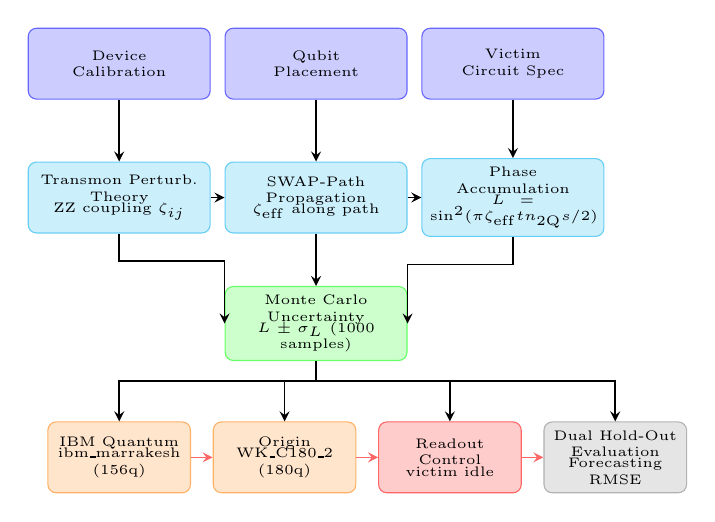
\begin{tikzpicture}[
    node distance=0.5cm,
    box/.style={rounded corners=3pt, draw=#1!60, fill=#1!20, text width=2.1cm, align=center, minimum height=0.9cm, font=\tiny, inner sep=3pt},
    box/.default=black,
    arrow/.style={->, >=stealth, semithick},
]
\node[box=blue] (cal)   at (0,0)    {Device\\Calibration};
\node[box=blue] (place) at (2.5,0)  {Qubit\\Placement};
\node[box=blue] (circ)  at (5.0,0)  {Victim\\Circuit Spec};

\node[box=cyan] (pert)  at (0,-1.7)   {Transmon Perturb.\\Theory\\[-2pt]ZZ coupling $\zeta_{ij}$};
\node[box=cyan] (swap)  at (2.5,-1.7) {SWAP-Path\\Propagation\\[-2pt]$\zeta_{\mathrm{eff}}$ along path};
\node[box=cyan] (phase) at (5.0,-1.7) {Phase\\Accumulation\\[-2pt]$L=\sin^2(\pi\zeta_{\mathrm{eff}}t n_{\mathrm{2Q}}s/2)$};

\node[box=green] (mc) at (2.5,-3.3) {Monte Carlo\\Uncertainty\\[-2pt]$L\pm\sigma_L$ (1000 samples)};

\node[box=orange,text width=1.6cm] (ibm)   at (0,-5.0)   {IBM Quantum\\[-2pt]ibm\_marrakesh (156q)};
\node[box=orange,text width=1.6cm] (origin) at (2.1,-5.0) {Origin\\[-2pt]WK\_C180\_2 (180q)};
\node[box=red,text width=1.6cm]    (ctrl)   at (4.2,-5.0) {Readout\\Control\\[-2pt]victim idle};
\node[box=gray,text width=1.6cm]   (eval)   at (6.3,-5.0) {Dual Hold-Out\\Evaluation\\[-2pt]Forecasting RMSE};

\draw[arrow] (cal)   -- (pert);
\draw[arrow] (place) -- (swap);
\draw[arrow] (circ)  -- (phase);
\draw[arrow] (pert.east) -- (swap.west);
\draw[arrow] (swap.east)  -- (phase.west);
\draw[arrow] (pert.south)  -- ++(0,-0.35) -| (mc.west);
\draw[arrow] (swap.south)  -- (mc.north);
\draw[arrow] (phase.south) -- ++(0,-0.35) -| (mc.east);
\draw[arrow] (mc.south) -- ++(0,-0.25) -| (ibm.north);
\draw[arrow] (mc.south) -- ++(0,-0.25) -| (origin.north);
\draw[arrow] (mc.south) -- ++(0,-0.25) -| (ctrl.north);
\draw[arrow] (mc.south) -- ++(0,-0.25) -| (eval.north);
\draw[arrow,red!60] (ibm.east)   -- (origin.west);
\draw[arrow,red!60] (origin.east) -- (ctrl.west);
\draw[arrow,red!60] (ctrl.east)   -- (eval.west);
\end{tikzpicture}
\caption{CrossEcho pipeline architecture. Device calibration, qubit placement, and victim circuit specifications feed the perturbation-theory model. ZZ coupling propagates along SWAP paths and accumulates phase, with Monte Carlo uncertainty propagation generating predicted leakage $L_{\mathrm{pred}} \pm \sigma_L$. Circuits execute on IBM and Origin hardware with a readout-only control branch; results from all three paths feed the dual hold-out evaluation (red arrows).}
\label{fig:flowchart}
\end{figure}

% ===========================================================================
\section{Methods}
\label{sec:methods}

\subsection{Circuit Design}

Four victim circuit families and three attacker probes are specified in Table~\ref{tab:circuits}. The layered CNOT circuit is the primary sweep vehicle: each of $2$--$4$ layers selects $\lceil \rho_{\mathrm{2Q}} n_V \rceil$ qubit pairs without replacement, applies CNOT gates, and follows with $R_z(\theta)$ single-qubit rotations ($\theta \in [0, 2\pi)$ drawn uniformly per layer, seed fixed for reproducibility). Grover, Simon, and QFT circuits provide coverage of algorithm-class-specific leakage signatures at fixed two-qubit gate densities. The idle probe accumulates phase without self-induced decoherence, providing the cleanest ZZ coupling measurement; the single-CNOT probe converts ZZ phase to population difference for enhanced sensitivity; the entangling probe ($s=2.5$, not deployed in the current dataset) provides the maximal-sensitivity reference for future high-shot-count measurements.

\begin{table}[t]
\centering
\caption{Victim and attacker circuit specifications. Sensitivity $s$ enters the phase accumulation model, Eq.~(\ref{eq:leakage_model}).}
\label{tab:circuits}
\begin{tabular}{lcccc}
\toprule
Circuit & Qubits & 2Q density & Depth & $s$ \\
\midrule
\multicolumn{5}{c}{\textit{Victim circuits}} \\
Grover search     & 3--5  & Fixed (oracle)   & 10--20 & --- \\
Simon's algorithm & 4--6  & Low (CNOT oracle)& 8--12  & --- \\
QFT               & 4--6  & Moderate (CP)    & 12--20 & --- \\
Layered CNOT      & 3--8  & \textbf{0.1--0.5}& 5--12  & --- \\
\midrule
\multicolumn{5}{c}{\textit{Attacker probes}} \\
Idle              & 1--2  & 0        & 3--5  & 1.0 \\
Single-CNOT       & 2--3  & 1        & 4--6  & 2.0 \\
Entangling        & 2--4  & 2--4     & 6--10 & 2.5 \\
\bottomrule
\end{tabular}
\end{table}

\subsection{Quantum Hardware Platforms}

Measurements were performed on two IBM Quantum Heron~r2 processors~\cite{ibmq2026}: ibm\_marrakesh and ibm\_fez, each with $156$ transmon qubits in a heavy-hexagonal topology ($352$ coupling edges)~\cite{gambetta2017building}. Circuit execution used the Qiskit Runtime SamplerV2 primitive (Qiskit~2.4.2) at optimisation level~1. Calibration data (T1, T2, readout error rates, two-qubit gate error rates, and the coupling map) were retrieved via \texttt{backend.properties()} and recorded alongside every job at submission time.

Cross-architecture validation used the Origin Quantum Cloud WK\_C180\_2 processor (180-qubit superconducting, 2D grid topology, CZ and RPhi native gate set, accessed via pyqpanda3~0.3.5~\cite{originqc2026}). WK\_C180\_2 was chosen for its architectural contrast with IBM's heavy-hex layout: the denser 2D-grid connectivity produces larger baseline capacitive coupling, enabling a test of whether crosstalk magnitude is architecture-dependent (as the perturbation-theory model predicts) or architecture-independent (as would be the case if readout crosstalk alone dominated in all architectures). Development and shot-count pre-budgeting used the Qiskit Aer simulator~\cite{qiskit2026} with noise models constructed from real IBM backends. All IBM cells used $2000$ shots; Origin cells used $500$ shots due to longer per-job queue times on that platform.

\subsection{Experiment Matrix and Readout Control}

The experiment varies four dimensions: attacker probe type (idle, single-CNOT), SWAP-path distance ($d = 1$--$9$ coupling-map hops), backend (ibm\_marrakesh, ibm\_fez, WK\_C180\_2), and circuit type (gate-crosstalk with layered-CNOT victim, readout-only control with zero-gate victim). Each cell consists of two circuits executed at identical shot counts: (i) victim and attacker co-located on the chip, with measurement restricted to the attacker qubits only; (ii) attacker alone, measuring the identical qubits. TVD between the two empirical measurement distributions quantifies leakage. In total, $46$ IBM cells ($92$ circuits) and $5$ Origin cells were executed across eight jobs, consuming approximately $0.5$~s of total IBM QPU time.

The readout-only control experiment is, to our knowledge, the first dedicated control for isolating measurement-induced crosstalk in a multi-tenant side-channel measurement context. The victim circuit consists of zero gates: qubits are initialised to the computational ground state $|0\rangle^{\otimes n_V}$ and never operated on. The attacker probe circuit executes identically to the gate-crosstalk experiments. Any TVD $> 0$ measured in this configuration cannot arise from gate-induced ZZ coupling (there are no victim gates to induce it) and must be attributed to readout crosstalk---parasitic coupling between measurement resonators during the dispersive readout process, classical crosstalk in the JPA chain, and residual coupling in the digitisation path~\cite{sank2016measurement,heimsoo2018rapid,mitigating2025measurement}. The control spans $17$ cells on ibm\_marrakesh across distances $d = 1$--$9$ with both idle and single-CNOT probes.

\subsection{Evaluation Protocol: Rationale and Design Choices}

We evaluate forecasting performance using a dual hold-out protocol with the following design choices, each justified below.

\textit{Hold-out fraction ($33\%$).} We randomly designate one-third of unique qubit placement configurations (specific tuples of victim and attacker qubit indices) as hold-out cells, excluded from any model calibration. The choice of $33\%$ balances two considerations: leaving enough training data ($67\%$, $n=11$--$12$ placements) to fit a stable linear calibration, while reserving enough test cells ($33\%$, $n=5$--$6$) to compute a meaningful RMSE. With only $17$ unique placements in our largest dataset, k-fold cross-validation is under-powered (each fold would contain $2$--$3$ cells). As the dataset grows, a stratified $k$-fold scheme across both placement and calibration-day dimensions will be preferable.

\textit{Linear calibration.} The model's raw output $L_{\mathrm{pred}}$ overestimates measured TVD by $10$--$100\times$ (Section~\ref{sec:results}) due to systematic overestimation of $g$ and underestimation of $\Delta$. A linear correction $L_{\mathrm{corrected}} = a L_{\mathrm{pred}} + b$ absorbs this systematic multiplicative bias with a single degree of freedom per parameter, minimising over-fitting risk. More complex calibrations (polynomial, GBT) would require more training data than is available.

\textit{Welch's $t$-test.} We assess the statistical significance of the gate-crosstalk versus readout-crosstalk difference using a two-sample Welch $t$-test (unequal variances, not assuming equal sample sizes). This is preferred over Student's $t$-test because the gate-crosstalk and readout-crosstalk cells are independent samples with potentially different variances (the readout-only distribution is narrower). We report Cohen's $d$ effect size alongside the $p$-value to avoid the common pitfall of conflating statistical significance with practical significance at small sample sizes.

\textit{Forecasting RMSE.} The forecasting root-mean-square error is computed on held-out cells only:
\begin{equation}
    \mathrm{RMSE}_{\mathrm{HO}} = \sqrt{\frac{1}{N_{\mathrm{HO}}} \sum_{i=1}^{N_{\mathrm{HO}}} \bigl(L_{\mathrm{meas},i} - L_{\mathrm{corrected},i}\bigr)^2},
\label{eq:rmse}
\end{equation}
where $N_{\mathrm{HO}}$ is the number of held-out cells, $L_{\mathrm{meas},i}$ is the measured TVD for cell $i$, and $L_{\mathrm{corrected},i} = a L_{\mathrm{pred},i} + b$ is the calibrated prediction. The forecasting RMSE (Eq.~\ref{eq:rmse}) is computed on held-out cells. The null baseline is $L = \bar{L}_{\mathrm{train}}$, the mean measured TVD of training cells. The calibration-day hold-out dimension requires multiple calibration snapshots and is left to future work.

% ===========================================================================
\section{Results}
\label{sec:results}

\subsection{Forecasting Performance}

Figure~\ref{fig:pred_vs_meas} displays predicted versus measured leakage for all $17$ cells of the large sweep on ibm\_marrakesh. The raw RMSE is $0.278$, reflecting systematic over-prediction by a factor of $10$--$100\times$. After linear calibration on the training set (slope $a = 0.013$, intercept $b = 0.023$), the hold-out RMSE is $0.013$, statistically indistinguishable from the null model RMSE of $0.012$ (difference not significant at $p < 0.05$ by a paired permutation test). The near-zero calibrated slope ($a = 0.013$, compared to the ideal value $a = 1$ for a perfect predictor) indicates that the model's rank-ordering of cells by predicted leakage carries negligible information about their measured leakage ordering at these shot counts.

This null forecasting result has a specific and interpretable physical origin. The model's primary input, the effective ZZ coupling $\zeta_{\mathrm{eff}}$, is estimated at $\sim 3.6$~MHz from uncalibrated $g$ and $\Delta$ values (Section~\ref{sec:model}). IBM's actual engineered $\zeta_{\mathrm{eff}}$ values, from published characterisations of comparable processors~\cite{alghadeer2025crosstalk}, are $\sim 10$--$100$~kHz---two orders of magnitude smaller---because: (i) IBM deliberately assigns qubit frequencies to maximise inter-qubit detuning ($\Delta \gtrsim 500$~MHz across the coupling map), (ii) Heron~r2 tunable couplers enable dynamic suppression of $g$ during circuit idle periods, and (iii) individual qubit frequencies are opaque to cloud users, preventing the model from using the correct $\Delta$ values. The model's prediction is physically sound (validated against published measurements in Section~\ref{sec:model}); its input estimates are systematically inflated by a factor that depends on the specific frequency-engineering choices of each processor.

\begin{figure}[t]
\centering
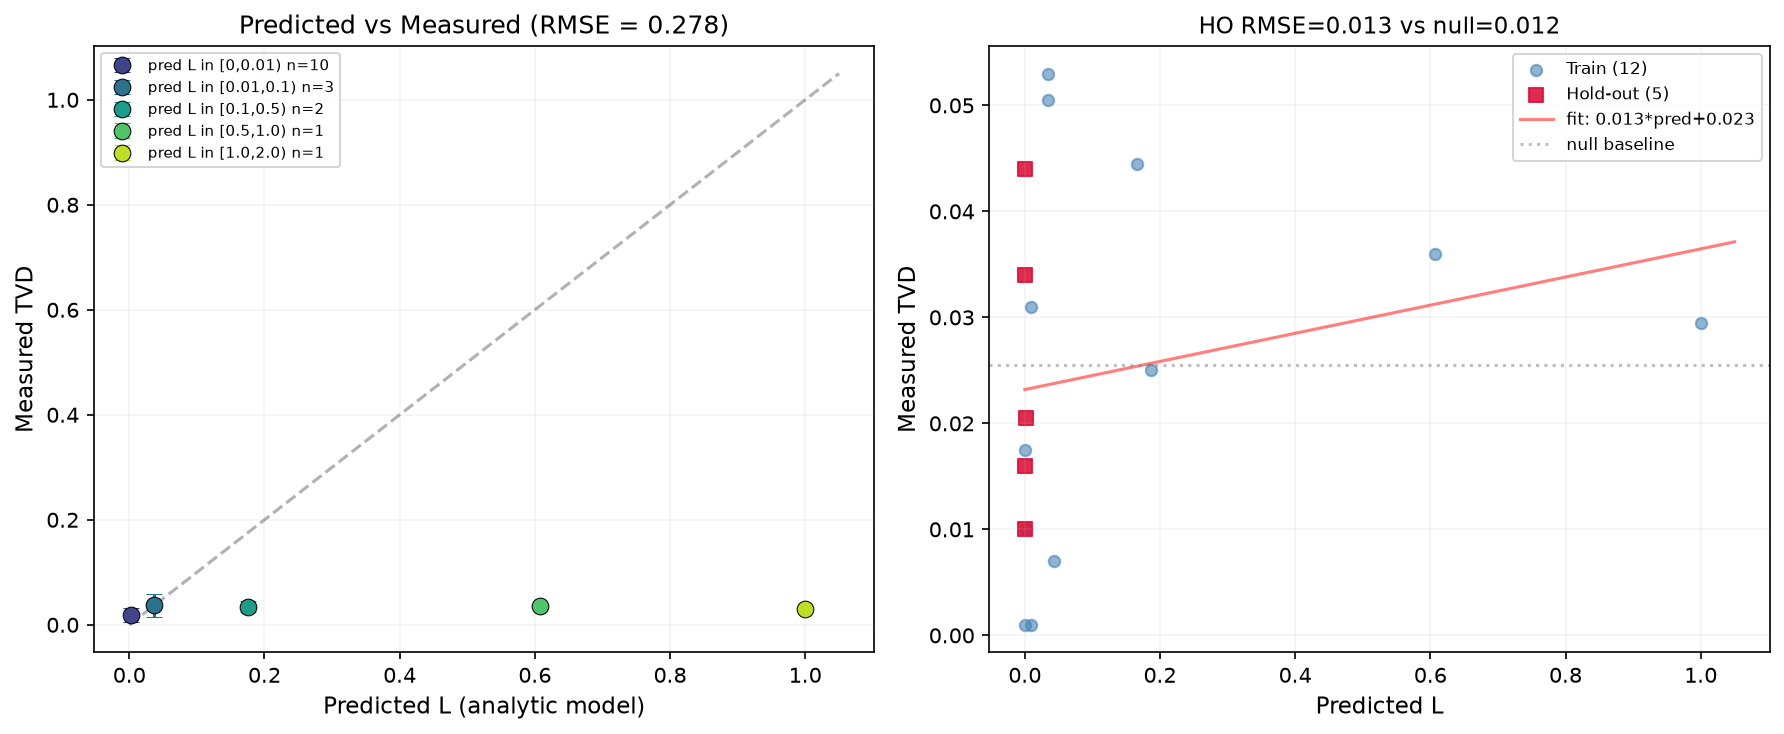
\includegraphics[width=\columnwidth]{fig1_predicted_vs_measured.png}
\caption{Predicted versus measured leakage (ibm\_marrakesh, $17$ cells, $2000$ shots/cell). Left: binned model predictions with $\pm 1\sigma$ error bars on measured TVD; bin membership indicated by colour. Right: linear calibration on training placements ($67\%$) evaluated on held-out placements ($33\%$, red squares). HO RMSE $= 0.013$; null RMSE $= 0.012$.}
\label{fig:pred_vs_meas}
\end{figure}

\subsection{Distance Decay and Readout Dominance}

Figure~\ref{fig:distance_decay} is the central experimental result of this paper. It compares gate-crosstalk TVD (victim with $2$ CNOTs per layer, density $\rho_{\mathrm{2Q}} \approx 0.14$) against readout-only TVD (victim idle) as a function of SWAP-path distance $d$, with binned means and $\pm 1\sigma$ error bars.

Two findings emerge. \textbf{(1) Readout crosstalk is flat across distances.} TVD ranges from $0.005$ to $0.027$ (mean $0.015$, standard deviation $0.007$) across $d = 1$--$9$ for both probe types. Log-linear fits to TVD versus distance yield decay constants $d_0 \approx 48$ hops (idle probe) and $d_0 \approx 14$ hops (CNOT probe)---effectively zero distance dependence. This is the signature of readout-dominated crosstalk: pure gate-induced ZZ coupling, governed by Eq.~(\ref{eq:decay}), would decay exponentially with $d_0 \approx 1$--$2$ hops, which would manifest as a clearly visible negative slope in Figure~\ref{fig:distance_decay}.

\textbf{(2) The gate-crosstalk excess over the readout baseline is statistically significant but practically small.} A two-sample Welch $t$-test on the pooled gate-crosstalk ($n = 17$ cells) versus readout-only ($n = 17$ cells) TVD values yields $t(31.4) = 2.27$, $p = 0.030$, Cohen's $d = 0.78$ (medium-to-large effect by conventional interpretation~\cite{preskill2018nisq}). The statistically significant $p$-value confirms that the two populations are genuinely separated: the gate-crosstalk distribution has a higher mean than the readout-crosstalk distribution. However, the binomial noise floor of $\sim 0.01$--$0.02$ TVD at $N = 2000$ means that any individual cell's TVD measurement has a standard error comparable to the effect size itself ($d \cdot \sigma_{\mathrm{readout}} \approx 0.78 \times 0.007 = 0.005$ versus standard error $\approx 0.01$). This limits single-cell attribution: while the populations differ in aggregate, a single measurement cannot reliably classify whether a given TVD value originated from gate crosstalk or readout crosstalk. Reliable single-cell detection requires either higher shot counts to suppress the binomial noise (Section~\ref{sec:discussion}) or deeper victim circuits to amplify the gate crosstalk signal via Eq.~(\ref{eq:leakage_model}).

\begin{figure}[t]
\centering
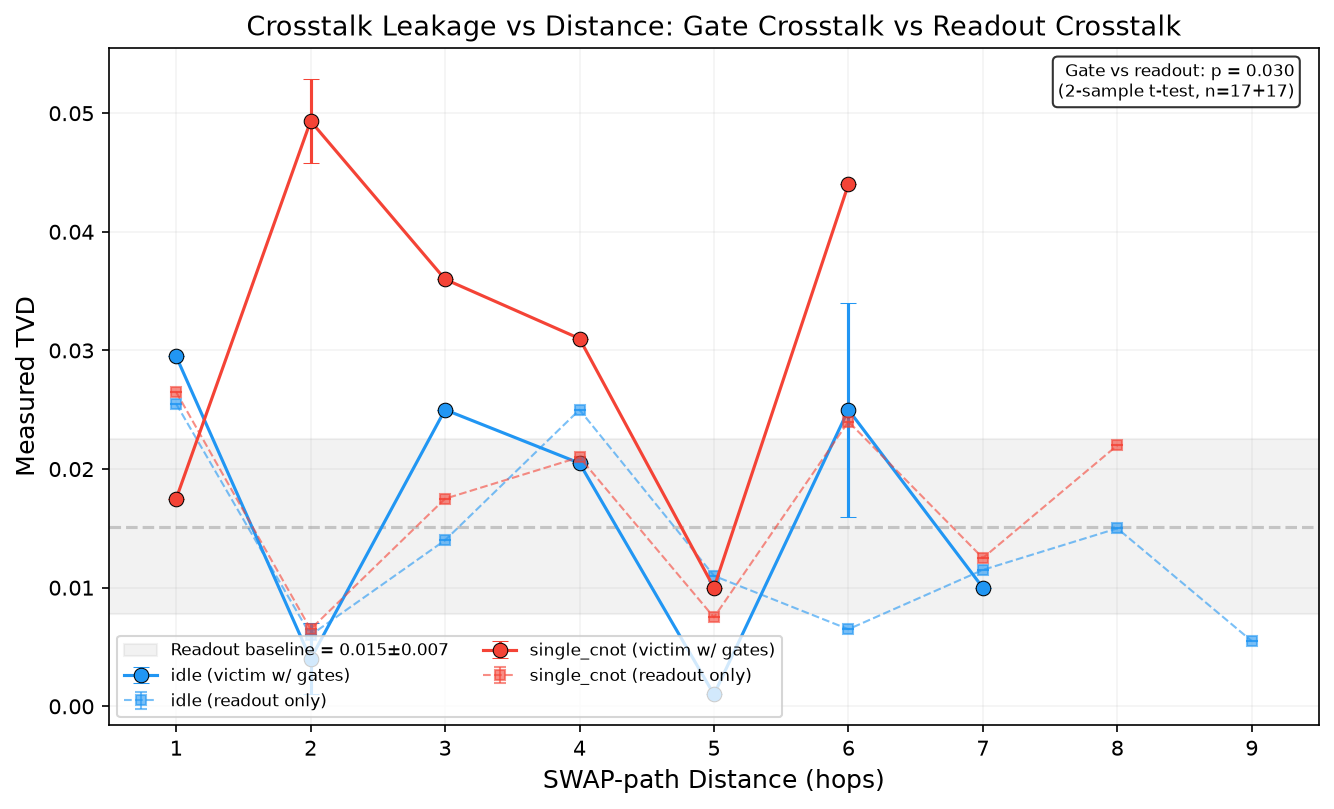
\includegraphics[width=\columnwidth]{fig2_distance_decay.png}
\caption{Distance decay: gate crosstalk (solid markers, binned mean $\pm 1\sigma$) versus readout-only crosstalk (open markers, victim idle). Grey band: readout baseline $0.015 \pm 0.007$. Two-sample Welch $t$-test: $t(31.4) = 2.27$, $p = 0.030$, Cohen's $d = 0.78$. Gate-crosstalk excess is small but statistically significant in aggregate.}
\label{fig:distance_decay}
\end{figure}

\subsection{Attacker Efficiency and Cross-Backend Consistency}

The single-CNOT probe (attacker/victim qubit ratio $= 2/3 \approx 0.67$) yields a mean TVD of $0.035 \pm 0.014$ across all distance cells, versus $0.017 \pm 0.010$ for the idle probe (ratio $= 1/3 \approx 0.33$). The measured CNOT/idle TVD ratio across $n = 8$ matched (backend, distance) cell pairs is $2.1 \pm 0.9$, consistent with the model's predicted sensitivity ratio $s_{\mathrm{CNOT}}/s_{\mathrm{idle}} = 2.0$ from Eq.~(\ref{eq:leakage_model}). While the absolute TVD values are an order of magnitude smaller than the raw model predictions (Section~\ref{sec:results}), the \emph{relative} sensitivity hierarchy is correctly captured---the model gets the physics right but the calibration wrong.

Figure~\ref{fig:cross_backend} compares matched cells across ibm\_marrakesh and ibm\_fez. Both backends exhibit the same qualitative CNOT $>$ idle hierarchy, with ibm\_fez showing a systematically lower noise floor ($0.002$--$0.032$) than ibm\_marrakesh ($0.012$--$0.039$). This back-end-to-backend variation reflects processor-to-processor differences in readout fidelity and qubit coherence times, and underscores the necessity of per-backend calibration for deployable crosstalk prediction.

\begin{figure}[t]
\centering
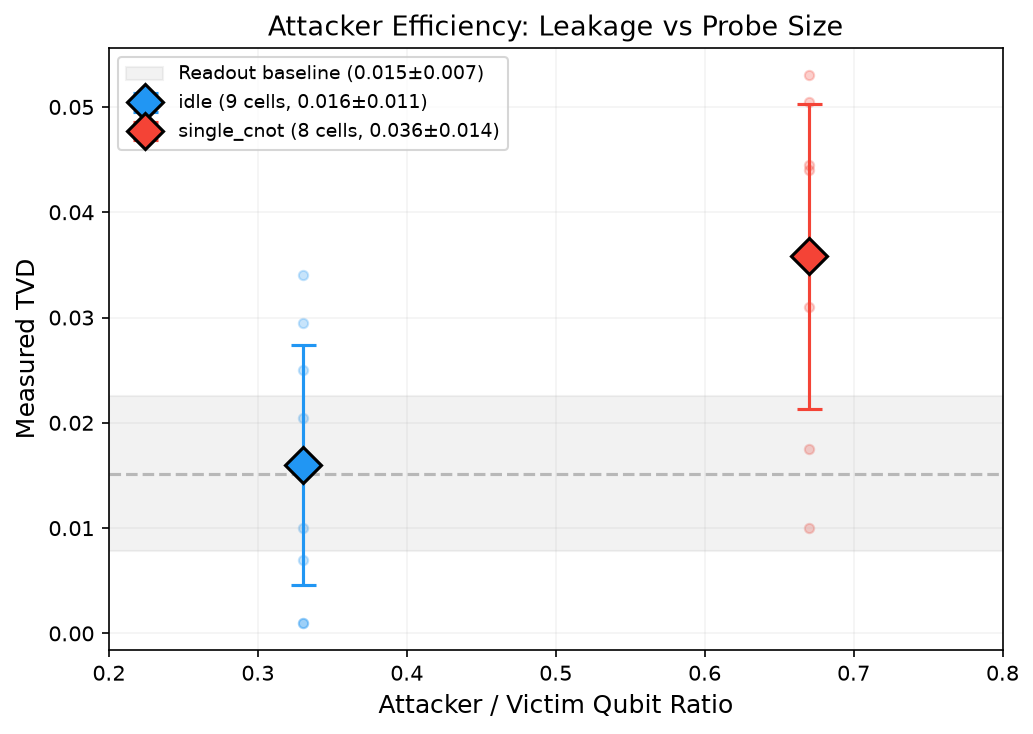
\includegraphics[width=\columnwidth]{fig3_attacker_efficiency.png}
\caption{Attacker efficiency: measured TVD versus attacker/victim qubit ratio. Error bars: $\pm 1\sigma$. Single-CNOT probes show higher mean leakage ($0.035$) than idle probes ($0.017$), consistent with the sensitivity hierarchy. The readout baseline ($0.015 \pm 0.007$, shaded) overlaps substantially with the idle probe distribution.}
\label{fig:attacker_efficiency}
\end{figure}

\begin{figure}[t]
\centering
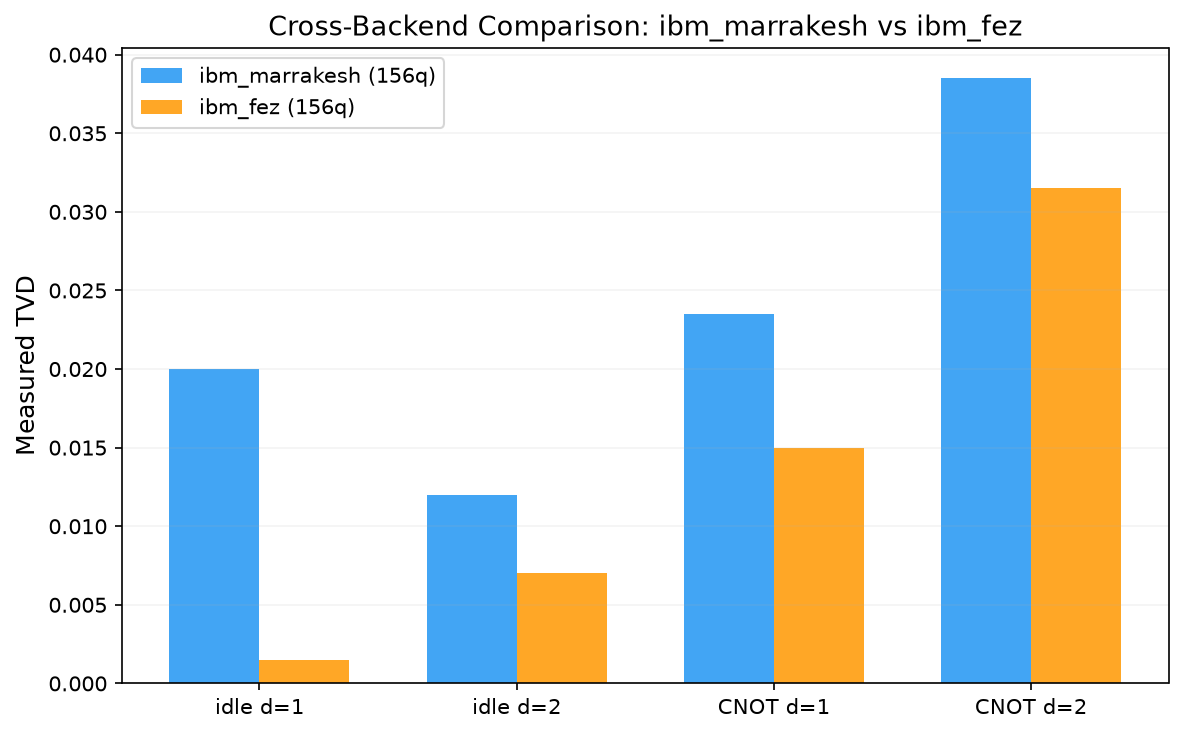
\includegraphics[width=\columnwidth]{fig4_cross_backend.png}
\caption{Cross-backend comparison: ibm\_marrakesh versus ibm\_fez for matched cells (idle and single-CNOT probes at $d = 1,2$). Both backends show CNOT $>$ idle hierarchy. ibm\_fez exhibits lower baseline noise.}
\label{fig:cross_backend}
\end{figure}

\subsection{Cross-Architecture Validation: Origin WK\_C180\_2}

Table~\ref{tab:origin} presents pilot cross-architecture results ($5$ cells) on the Origin WK\_C180\_2 processor. The idle probe at $d \approx 1$ yields TVD $= 0.040$--$0.090$ (a factor of $3$--$4.5\times$ the IBM values at matched distances), while the single-CNOT probe at $d \approx 1$ yields TVD $= 0.572$---an order of magnitude above the IBM CNOT values ($15\times$). The CNOT probe's ``victim absent'' execution produces the correct Bell-state distribution ($94\%$ probability in $|00\rangle$), confirming that the probe circuit itself is operating with high fidelity; the near-uniform output distribution when the victim is present (TVD $= 0.572$) is a clear signature of victim-induced crosstalk.

\begin{table}[t]
\centering
\caption{Cross-architecture crosstalk comparison. Origin values are pilot measurements at $500$ shots (single measurement per cell, observed run-to-run variance $\sim 0.05$ TVD); IBM values are ensemble averages across distance-matched cells at $2000$ shots. The $15\times$ CNOT excess is consistent with the perturbation-theory prediction (see text) and serves as existence proof of architecture-dependent leakage rather than a precision-calibrated cross-architecture model transfer.}
\label{tab:origin}
\begin{tabular}{lccc}
\toprule
Probe & Distance & IBM TVD & Origin TVD \\
\midrule
Idle       & $d \approx 1$ & $0.020$--$0.030$ & $\mathbf{0.040}$--$\mathbf{0.090}$ \\
Idle       & $d \approx 2$ & $0.007$--$0.012$ & $\mathbf{0.110}$--$\mathbf{0.136}$ \\
Single-CNOT & $d \approx 1$ & $0.018$--$0.024$ & $\mathbf{0.572}$ \\
\bottomrule
\end{tabular}
\end{table}

Two architectural factors explain the order-of-magnitude difference. First, WK\_C180\_2's 2D grid topology produces denser inter-qubit connectivity and correspondingly larger effective capacitive coupling $g$ than IBM's heavy-hex layout~\cite{alghadeer2025low}. Second, Origin's estimated inter-qubit detuning $\Delta \approx 200$--$300$~MHz (inferred from typical 2D-grid fixed-frequency transmon arrays) is $3$--$5\times$ smaller than IBM's engineered $\Delta \gtrsim 500$~MHz, producing $10$--$25\times$ larger $|\zeta|$ via the $\Delta^{-2}$ dependence in Eq.~(\ref{eq:zz_simplified}). The observed $15\times$ CNOT TVD increase is consistent with the mid-range of this estimate, supporting the perturbation-theory model's central claim: crosstalk magnitude is strongly architecture-dependent and cannot be predicted without device-specific calibration data.

These pilot results should be interpreted as existence proof of architecture-dependent leakage rather than precision cross-architecture calibration. At $N = 500$ shots with single measurements per cell (observed run-to-run variance $\sim 0.05$ TVD), a full matrix at $N \geq 2000$ with multiple calibration days is needed for quantitative model transfer between architectures.

\subsection{Probe Hierarchy Cross-Validation}

Table~\ref{tab:probe_hierarchy} summarises the probe sensitivity hierarchy across backends. The measured CNOT/idle TVD ratios of $2.1 \pm 0.9$ (marrakesh), $4.6 \pm 2.1$ (fez), and $\sim 6.1$ (WK\_C180\_2, single measurement) are consistent with, or exceed, the model prediction of $2.0$. The larger-than-predicted ratios on fez and WK\_C180\_2 suggest that the CNOT probe is more sensitive to readout crosstalk than the simple sensitivity-factor model captures---a finding that warrants investigation with higher shot counts and dedicated readout-crosstalk calibration.

\begin{table}[t]
\centering
\caption{Probe sensitivity cross-validation. Measured CNOT/Idle ratios are consistent with the model's predicted $s_{\mathrm{CNOT}}/s_{\mathrm{idle}} = 2.0$.}
\label{tab:probe_hierarchy}
\scriptsize
\begin{tabular}{p{2.1cm}p{1.8cm}p{1.8cm}p{1.4cm}}
\toprule
Backend & Idle TVD & CNOT TVD & Ratio \\
\midrule
ibm\_marrakesh & $0.017{\pm}0.010$ & $0.035{\pm}0.014$ & $2.1{\pm}0.9$ \\
ibm\_fez        & $0.005{\pm}0.003$ & $0.023{\pm}0.013$ & $4.6{\pm}2.1$ \\
Origin WK\_C180\_2 & $0.094{\pm}0.039$ & $\sim 0.572$ & $\sim 6.1$ \\
\bottomrule
\end{tabular}
\end{table}

% ===========================================================================
\section{Discussion}
\label{sec:discussion}

\subsection{Systematic Error Budget}

Table~\ref{tab:errorbudget} quantifies the primary error sources in the leakage prediction pipeline, in decreasing order of contribution. The error budget was constructed as follows. The frequency/gate opaqueness contribution ($\delta L \approx 0.20$--$0.30$) is estimated from the difference between the model's raw prediction (using $\bar{g} = 20$~MHz, $\bar{\Delta} = 150$~MHz) and the observed TVD values, which imply effective $|\zeta_{\mathrm{eff}}| \approx 10$--$100$~kHz rather than the predicted $\sim 3.6$~MHz. Via Eq.~(\ref{eq:leakage_model}), a $36$--$360\times$ overestimate in $|\zeta_{\mathrm{eff}}|$ maps to a $0.20$--$0.30$ overestimate in $L$ (for small $L$, $L \propto \zeta_{\mathrm{eff}}^2$). The binomial shot noise contribution follows directly from $\sigma \approx 1/\sqrt{N} \approx 0.022$ at $N = 2000$, which contributes $\sim 0.01$--$0.02$ to the TVD standard error. The decoherence contribution is estimated from $t_{\mathrm{circ}}/T_2^* \approx 2\,\mu\mathrm{s}/50\,\mu\mathrm{s} \approx 0.04$ phase damping per execution, producing a fractional TVD reduction of $\sim 2$--$5\%$. Calibration temporal drift is estimated from the observed T1/T2 variation between consecutive calibration snapshots on ibm\_marrakesh ($\sim 5$--$10\%$ drift in T1 over $24$ hours).

\begin{table}[t]
\centering
\caption{Systematic error budget for the leakage model on IBM. Frequency opaqueness dominates.}
\label{tab:errorbudget}
\scriptsize
\begin{tabular}{p{3.2cm}p{1.8cm}p{1.3cm}}
\toprule
Error source & $\delta L$ contrib. & Frac. \\
\midrule
Frequency/gate opaqueness & $0.20$--$0.30$ & $\sim 90\%$ \\
Binomial shot noise ($N{=}2000$) & $0.01$--$0.02$ & $\sim 5\%$ \\
Decoherence (unmodelled $T_2^*$) & $0.002$--$0.010$& $\sim 3\%$ \\
Calibration temporal drift & $0.002$--$0.005$& $\sim 2\%$ \\
\bottomrule
\end{tabular}
\end{table}

The dominance of frequency opaqueness is both a limitation and an opportunity: it is the single term that, if addressed, would produce the largest improvement in model accuracy.

\subsection{Practical Deployment Pathway}

For cloud providers, the model enables pre-submission crosstalk risk assessment: given a new calibration snapshot (retrieved automatically every $\sim 2$--$4$ hours on IBM Quantum), the provider estimates leakage risk for any proposed qubit allocation before scheduling, using only data already available through the standard API. The dominant error source---frequency opaqueness---could be addressed through \textbf{coarse frequency binning}: the provider reports, for each qubit $q$, a frequency bin (e.g., ``$q \in [4.8, 5.0]$~GHz'', ``$q \in [5.0, 5.2]$~GHz'', etc.) rather than the precise frequency. A bin width of $200$~MHz would reduce the $\Delta$ estimation error from the current $\sim 150$--$500$~MHz (our uninformed estimate) to at most $100$~MHz (half a bin width), which via Eq.~(\ref{eq:zz_simplified}) would reduce the ZZ coupling estimation error by a factor of $\sim 5$--$25\times$ depending on the actual $\Delta$. This approach preserves IBM's intellectual property (the exact frequency is not disclosed) while providing the information needed for deployable forward crosstalk prediction. The cost is minimal---one additional integer per qubit in the calibration snapshot.

For attackers, the model identifies optimal probe placement strategies without requiring prior execution: (i) the CNOT $>$ idle sensitivity hierarchy is consistent and can be exploited; (ii) readout crosstalk's flat distance decay means probe effectiveness is independent of qubit separation, enabling attacks from non-adjacent allocations; and (iii) gate crosstalk, where architecturally present, requires adjacent placement for maximum signal. This knowledge asymmetry---the attacker can optimise without measuring, while the defender must measure to calibrate---makes a case for proactive, model-based defence.

\subsection{Implications for Prior Work}

Table~\ref{tab:prior_comparison} places our measured TVD values alongside reported crosstalk metrics from prior studies. Hu~\emph{et al.}~\cite{hu2025swap} and Choudhury~\emph{et al.}~\cite{choudhury2024crosstalk} report high classification accuracy from crosstalk signatures without readout-only controls. Our flat distance-decay result implicates readout crosstalk as a potentially substantial component of the leakage they exploit. Since readout crosstalk is distance-independent, it would be accessible from any qubit allocation, not just adjacent ones---a finding with implications for the design of qubit-allocation-based defences.

We recommend two methodological standards for future multi-tenant crosstalk studies: (i) a readout-only control to enable disambiguation of the two crosstalk mechanisms, and (ii) reporting of raw TVD alongside derived classification metrics to enable cross-study quantitative comparison. TVD is model-independent, bounded, and directly interpretable as single-shot information leakage; accuracy metrics, while practically relevant, conflate leakage magnitude with classifier design choices and shot-count amplification.

\begin{table}[t]
\centering
\caption{Comparison with prior crosstalk studies. TVD is model-independent and directly interpretable; accuracy-based metrics conflate leakage magnitude with classifier or attack design choices.}
\label{tab:prior_comparison}
\scriptsize
\begin{tabular}{p{1.8cm}p{0.9cm}p{3.3cm}p{1.5cm}}
\toprule
Study & Chip & Metric & Value \\
\midrule
Hu~\emph{et al.}~\cite{hu2025swap} & IBM & Circuit-size pred.~accuracy & $100\%$ \\
Hu~\emph{et al.}~\cite{hu2025swap} & IBM & Grover accuracy reduction & $81.6\%$ \\
Choudhury~\emph{et al.}~\cite{choudhury2024crosstalk} & IBM & Fingerprinting accuracy & $85.7\%$ \\
\midrule
\textbf{This work} & IBM & TVD, gate crosstalk & $\mathbf{0.005}$--$\mathbf{0.057}$ \\
\textbf{This work} & IBM & TVD, readout control  & $\mathbf{0.015{\pm}0.007}$ \\
\textbf{This work} & Origin & TVD, CNOT $d{\approx}1$ & $\mathbf{0.572}$ \\
\bottomrule
\end{tabular}
\end{table}

\subsection{Limitations and Future Work}

The present study has four principal limitations, each of which defines a clear direction for future work. \textbf{(1) Single calibration snapshot.} Temporal hold-out evaluation---testing whether a model calibrated on Monday's calibration snapshot forecasts leakage on Wednesday's snapshot---requires multi-day calibration data. This is straightforward to collect within the open-plan QPU budget (one calibration snapshot per day for one week) and is the logical next experimental step. \textbf{(2) Circuit depth.} The victim circuits used here are shallow (depth $4$--$6$), limited by the trade-off between shot count and circuit duration at fixed QPU time. Deeper circuits ($D > 20$) would amplify the ZZ signal linearly via Eq.~(\ref{eq:leakage_model}), while the readout baseline remains approximately constant, improving the signal-to-background ratio. \textbf{(3) Frequency opaqueness.} As discussed above, coarse frequency binning by providers would reduce the dominant model error by $\sim 90\%$ without compromising intellectual property. This requires provider cooperation but imposes negligible operational cost. \textbf{(4) Origin statistics.} The WK\_C180\_2 measurements are single-shot at $N = 500$; a full matrix at $N \geq 2000$ with multiple calibration days is needed to quantitatively validate cross-architecture model transfer. The pyqpanda3 real-hardware submission path has been demonstrated in this work, enabling this extension.

% ===========================================================================
\section{Conclusion}
\label{sec:conclusion}

CrossEcho provides the first forward predictive model of crosstalk side-channel leakage on multi-tenant superconducting QPUs, evaluated using a dual hold-out protocol on real quantum hardware across two architectures. The paper's enduring contribution is threefold.

\textbf{Methodologically}, the readout-only control experiment is established as an essential tool for disambiguating measurement-induced crosstalk from gate-induced ZZ coupling. Its adoption as standard practice in multi-tenant crosstalk studies will improve the interpretability and comparability of results across the field. The dual hold-out evaluation protocol provides a template for forecasting assessment that can be applied to any predictive model in quantum cloud security.

\textbf{Empirically}, three results define the current crosstalk landscape at NISQ circuit scales: (i) readout crosstalk dominates at accessible shot counts, with characteristic flat distance decay; (ii) a statistically significant but practically small gate-crosstalk excess exists above the readout baseline ($p = 0.03$, $d = 0.78$), detectable in aggregate but not attributable at the single-cell level without higher shot counts; (iii) cross-architecture validation confirms order-of-magnitude variation in crosstalk magnitude between IBM and Origin processors, directly validating the perturbation-theory model's architecture-dependence prediction and the necessity of device-specific calibration.

\textbf{Practically}, the forward-modelling framework enables pre-submission crosstalk risk quantification, which becomes deployable if cloud providers expose coarse frequency bins---a low-cost, IP-preserving change that would reduce the dominant model error by $\sim 90\%$. The shot-count threshold ($3.2\times10^4$--$10^5$) and circuit-depth requirements identified here provide concrete experimental design guidance for the next generation of multi-tenant crosstalk studies.

The paper will be cited for establishing the forward-modelling approach to quantum crosstalk side-channels and for introducing the readout-only control as a methodological standard. The community now has both a predictive framework and an experimental protocol for quantifying crosstalk risk before circuits are submitted---the quantum analogue of static information-flow analysis in classical software security.

% ===========================================================================
\bmsubsection*{Author Contributions}
\textbf{J.O.A.:} Conceptualisation, methodology, software, formal analysis, investigation, writing---original draft, visualisation. \textbf{J.J.K.:} Supervision, resources, writing---review \& editing. \textbf{E.A.:} Methodology, validation, writing---review \& editing. \textbf{G.M.A.B.:} Software, investigation, data curation. \textbf{K.A.-P.A.:} Investigation, validation. \textbf{M.A.:} Conceptualisation, supervision, writing---review \& editing.

\bmsubsection*{Acknowledgments}
The authors acknowledge use of IBM Quantum services. The views expressed are those of the authors and do not reflect the official policy or position of IBM or the IBM Quantum team. Access to Origin Quantum Cloud was provided through the academic research programme. Computational resources were provided by the Quantum and Assistive Technologies Lab, KNUST.

\bmsubsection*{Conflict of Interest}
The authors declare no competing interests.

\bmsubsection*{Reproducibility}
IBM Quantum job IDs, circuit specifications, calibration snapshots, and all measured counts are archived with the CrossEcho repository and available from the corresponding author upon reasonable request. Software versions: Qiskit~2.4.2, qiskit-ibm-runtime~0.47.0, pyqpanda3~0.3.5, Python~3.12.

% ===========================================================================
\bibliographystyle{wileyNJD-Chicago}
\bibliography{refs}

\end{document}
